% LaTeX Präsentationsvorlage (2013) der TU Graz, rev12, 2013/01/31
% !TeX encoding = UTF-8
\documentclass{beamer}
% \documentclass[aspectratio=169]{beamer}
% \usetheme{tugraz2013}
% \usetheme[notes]{tugraz2013}
\usepackage{../common/beamerthemetugraz2013}
\usepackage{color}
\usepackage{multicol}
\usepackage{bbding}
\usepackage{wasysym}
\usepackage{caption}
\usepackage{array}
% \usepackage{minted}

\usepackage{listings}
\usepackage{xcolor}

\definecolor{codegreen}{rgb}{0,0.6,0}
\definecolor{codegray}{rgb}{0.5,0.5,0.5}
\definecolor{codepurple}{rgb}{0.58,0,0.82}
\definecolor{backcolour}{rgb}{0.95,0.95,0.92}
\lstdefinestyle{mystyle}{
    backgroundcolor=\color{backcolour},   
    commentstyle=\color{codegreen},
    keywordstyle=\color{magenta},
    numberstyle=\tiny\color{codegray},
    stringstyle=\color{codepurple},
    basicstyle=\ttfamily\footnotesize,
    breakatwhitespace=false,         
    breaklines=true,                 
    captionpos=b,                    
    keepspaces=true,                 
    numbers=left,                    
    numbersep=5pt,                  
    showspaces=false,                
    showstringspaces=false,
    showtabs=false,                  
    tabsize=2
}

\lstset{style=mystyle}

\usepackage{picture}
\usepackage{rotating}
\definecolor{darkred}{rgb}{0.85,0.16,0.0}
\definecolor{darkgreen}{rgb}{0.16,0.70,0.27}

\usepackage{xcolor}


\newcommand{\hrefu}[2]{\underline{\href{#1}{#2}}}
\newcommand{\hyperlinku}[2]{\underline{\hyperlink{#1}{#2}}}
\newcommand{\smallurl}[1]{%
  \begin{flushleft}
    \tiny\url{#1}
  \end{flushleft}
}
\newcommand{\smalltext}[1]{%
  \begin{flushleft}
    \tiny{#1}
  \end{flushleft}
}
\newcommand{\red}[1]{{\color{red} #1}}
\newcommand{\blue}[1]{{\color{blue} #1}}
\newcommand{\darkgreen}[1]{\textcolor{darkgreen}{#1}}
\newcommand{\darkred}[1]{\textcolor{darkred}{#1}}

\newcommand*{\vpointer}{\vcenter{\hbox{\scalebox{1.5}{\large\pointer}}}}

\newcommand{\be}[1]{\begin{equation} \label{#1}}
\newcommand{\ee}{\end{equation}}
\newcommand{\bea}[1]{\begin{eqnarray} \label{#1}}
\newcommand{\eea}{\end{eqnarray}}
\newcommand{\bean}{\begin{eqnarray*}}
\newcommand{\eean}{\end{eqnarray*}}

\newcommand{\non}{\nonumber\\}
\newcommand{\eq}[1]{(\ref{#1})}
\newcommand{\difp}[2]{\frac{\partial #1}{\partial #2}}
\newcommand{\br}{{\bf r}}
\newcommand{\bR}{{\bf R}}
\newcommand{\bA}{{\bf A}}
\newcommand{\bB}{{\bf B}}
\newcommand{\bE}{{\bf E}}
\newcommand{\bm}{{\bf m}}
%\renewcommand{\bm}{{\bf m}}
\newcommand{\bn}{{\bf n}}
\newcommand{\bN}{{\bf N}}
\newcommand{\bp}{{\bf p}}
\newcommand{\bP}{{\bf P}}
\newcommand{\bF}{{\bf F}}
\newcommand{\by}{{\bf y}}
\newcommand{\bz}{{\bf z}}
\newcommand{\bZ}{{\bf Z}}
\newcommand{\bV}{{\bf V}}
\newcommand{\bv}{{\bf v}}
\newcommand{\bu}{{\bf u}}
\newcommand{\bx}{{\bf x}}
\newcommand{\bX}{{\bf X}}
\newcommand{\bW}{{\bf W}}
\newcommand{\bJ}{{\bf J}}
\newcommand{\bj}{{\bf j}}
\newcommand{\bk}{{\bf k}}
\newcommand{\bTheta}{{\bf \Theta}}
\newcommand{\btheta}{{\boldsymbol\theta}}
\newcommand{\bOmega}{{\bf \Omega}}
\newcommand{\bomega}{{\boldsymbol\omega}}
\newcommand{\brho}{{\boldsymbol\rho}}
\newcommand{\rd}{{\rm d}}
\newcommand{\rJ}{{\rm J}}
\newcommand{\ph}{{\varphi}}
\newcommand{\te}{\theta}
\newcommand{\tht}{\vartheta}
\newcommand{\vpar}{v_\parallel}
\newcommand{\vparkb}{v_{\parallel k b}}
\newcommand{\vparkm}{v_{\parallel k m}}
\newcommand{\Jpar}{J_\parallel}
\newcommand{\ppar}{p_\parallel}
\newcommand{\Bpstar}{B_\parallel^*}
\newcommand{\intpi}{\int\limits_{0}^{2\pi}}
\newcommand{\summ}{\sum \limits_{m=-\infty}^\infty}
\newcommand{\tb}{\tau_b(\uv)}
\newcommand{\bh}{{\bf h}}
\newcommand{\cE}{{\cal E}}
\newcommand{\bsigma}{{\boldsymbol\sigma}}
\newcommand{\bS}{{\mathbf S}}
\newcommand{\bI}{{\mathbf I}}
\newcommand{\odtwo}[2]{\frac{\rd #1}{\rd #2}}
\newcommand{\pdone}[1]{\frac{\partial}{\partial #1}}
\newcommand{\pdtwo}[2]{\frac{\partial #1}{\partial #2}}
\newcommand{\ds}{\displaystyle} % commands


%% Titelblatt-Einstellungen
\title[]
{Python 09}
\author[E.~Wachmann]{\scriptsize Elias Wachmann
}
\date{2024} % \today für heutiges Datum verwenden
\institute[Institute of Theoretical and Computational Physics]
{
}
\instituteurl{www.tugraz.at}
% \institutelogo{kurz.pdf}
%~ \additionallogo{merged_logos}
\AtBeginSection[]{
  \begin{frame}
  \vfill
  \centering
  \begin{beamercolorbox}[sep=8pt,center,shadow=true,rounded=true]{title}
    \usebeamerfont{title}\insertsectionhead\par%
  \end{beamercolorbox}
  \vfill
  \end{frame}
}
\lstset{
    literate={Ö}{{\"O}}1
             {Ä}{{\"A}}1
             {Ü}{{\"U}}1
             {ß}{{\ss}}1
             {ü}{{\"u}}1
             {ä}{{\"a}}1
             {ö}{{\"o}}1
}

%%%%%%%%%%%%%%%%%%%%%%%%%%%%%%%%%%%%%%%%%%%%%%%%%%%%%%%%%%%%%%%%%%%%%%%%%%%%
\begin{document}
%%%%%%%%%%%%%%%%%%%%%%%%%%%%%%%%%%%%%%%%%%%%%%%%%%%%%%%%%%%%%%%%%%%%%%%%%%%%
\titleframe

%\begin{frame}
%  \frametitle{Outline}
%  \tableofcontents%[hideallsubsections] 
%  \note{
%  	Meine Präsentation ist wie folgt strukturiert \ldots
%  }
%\end{frame}

\section*{Content}

\begin{frame}
\frametitle{Content}
  \tableofcontents
\end{frame}

%%%%%%%%%%%%%%%%%%%%%%%%%%%%%%%%%%%%%%%%%%%%%%%%%%%%%%%%%%%%%%%%%%%%%%%%%%%%
\section{Solving Linear Systems in Python}
\begin{frame}
  \frametitle{Numpy \texttt{linalg.solve}}
  \hrefu{https://numpy.org/doc/stable/reference/generated/numpy.linalg.solve.html}{\texttt{numpy.linalg.solve}} solves a linear matrix equation, or system of linear scalar equations of the form: 
  \begin{align}
    \mathbf{A} \mathbf{x} = \mathbf{b}
  \end{align}
  where $\mathbf{A}$ is a square matrix and $\mathbf{b}$ is a vector.\\
\end{frame}
\begin{frame}
  \frametitle{Numpy \texttt{linalg.solve}}
  \lstinputlisting[language=python]{examples/solve.py}
\end{frame}

\section{Solving DEs and Eigenvalue-Problems in Python}
\begin{frame}
  \frametitle{Scipy \texttt{scipy.integrate.solve\_ivp}}
  To solve initial value the \hrefu{https://docs.scipy.org/doc/scipy/reference/generated/scipy.integrate.solve_ivp.html}{solve\_ivp} function from the \hrefu{https://docs.scipy.org}{scipy} can be used. 
  
  \texttt{scipy.integrate.solve\_ivp(fun, t\_span, y0, method='RK45', t\_eval=None, dense\_output=False, events=None, vectorized=False, args=None)}

\end{frame}
\begin{frame}
  \frametitle{Scipy \texttt{scipy.integrate.solve\_ivp}}
  \begin{itemize}
    \item \texttt{fun}: function of DE. fun takes 2 args
    \item \texttt{t\_span}: tuple \((t_0, t_f)\) $\rightarrow$ integration intervall
    \item \texttt{y0}: initial conditions (array of initial values)
    \item \texttt{method}: Integration-method (defaults to 'RK45')
    \item \texttt{t\_eval}: Array of timesteps where sol is stored (opt.)
    \item \dots
  \end{itemize}
  
\end{frame}
\begin{frame}
  \frametitle{Scipy \texttt{scipy.integrate.solve\_ivp}}
  \lstinputlisting[language=python, firstline=3, lastline=14]{examples/ode.py}
\end{frame}
\begin{frame}
  \frametitle{Numpy \texttt{linalg.eig}}
To calculated the eigenvalues and eigenvectors for a given square matrix, the \texttt{numpy.linalg.eig} function can be used. 
\texttt{numpy.linalg.eig(a)}
\begin{itemize}
  \item Input: a \dots square matrix
  \item Output: (eigenvalues, eigenvectors) \dots named tuple with eigenvalues and eigenvectors
\end{itemize}
\end{frame}

\section{Further numpy specialties/functions}
\begin{frame}
  \frametitle{Numpy @-operator}
Starting with \texttt{python 3.5} \texttt{numpy} has a build-in operator for matrix multiplication. \\
\hspace{5mm}\\
\noindent \textbf{Note:} The \texttt{*}-operator does not matrix-multiply two 2D-arrays ($\rightarrow$ matrices)! It can be used to multiply \underline{element-wise}.\\
\hspace{5mm}\\
\noindent To actually perform matrix mutliplication the \texttt{@}-operator should be used.
\end{frame}
\begin{frame}
  \frametitle{Dot - products}
The \hrefu{https://numpy.org/doc/stable/reference/generated/numpy.dot.html}{numpy.dot} function calculates a dot product for two given arrays. \\
\hspace{5mm}\\
It may also be used to multiply two 0-D arrays (meaning numbers) or to multiply 2-D arrays (matrices). However, the \texttt{*}- and \texttt{@}-operators are preferred.
\end{frame}
\section{How do Computers communicate}
\begin{frame}
  \frametitle{How do Computers communicate?}
  Computers can communicate with other remote computer by using:\\
  \begin{itemize}
    \item \textbf{\hrefu{https://en.wikipedia.org/wiki/Ethernet}{Ethernet}}: Used to connect computers in a local network.
    \item \textbf{\hrefu{https://en.wikipedia.org/wiki/Wi-Fi}{WiFi}}: Wireless Fidelity. Used to connect computers in a local network.
    \item \textbf{\hrefu{https://en.wikipedia.org/wiki/Transmission_Control_Protocol}{TCP}/\hrefu{https://en.wikipedia.org/wiki/User_Datagram_Protocol}{UDP}}: Transmission Control Protocol / User Datagram Protocol. Used to transfer data over the internet.
    \item \textbf{\hrefu{https://en.wikipedia.org/wiki/Hypertext_Transfer_Protocol}{HTTP}}: HyperText Transfer Protocol. Used to transfer web pages.
  \end{itemize}
\end{frame}

\begin{frame}
  
  \begin{center}
    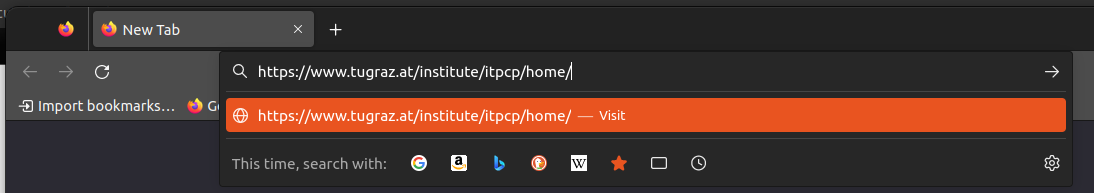
\includegraphics[width=\textwidth]{fig/search.png}
  \end{center}
  \begin{center}
    $\downarrow$ How does this work? $\downarrow$
  \end{center}
  \begin{center}
    \includegraphics[width=\textwidth]{fig/search\_result.png}
  \end{center}
\end{frame}
\begin{frame}
  \begin{center}
    \includegraphics[width=0.6\textwidth]{fig/osi\_model.png}
  \end{center}
  \vspace{-6mm}
  \smallurl{https://en.wikipedia.org/wiki/OSI\_model}
\end{frame}
\begin{frame}
  \frametitle{Let's look at a simplified example:}
  We want to access \texttt{\hrefu{www.tugraz.at/institute/itpcp/}{www.tugraz.at/institute/itpcp/}}\\
  \vspace{5mm}
  Our browser will send a \textbf{request} to the server at \texttt{\hrefu{www.tugraz.at}{www.tugraz.at}} using the \textbf{\hrefu{https://en.wikipedia.org/wiki/Hypertext_Transfer_Protocol}{HTTP}} protocol.\\
  \vspace{5mm}
  But how does he know where to send the request?\\
  \vspace{5mm}
  Computers have addresses, just like houses. They are called \textbf{\hrefu{https://en.wikipedia.org/wiki/IP\_address}{IP addresses}}.\footnote[frame]{\tiny actually it's more involved especially with IPv4 addresses $\rightarrow$ \hrefu{https://en.wikipedia.org/wiki/IPv4_address_exhaustion}{IPv4-exhaustion}}\\ % :( simplified i guess
\end{frame}
\begin{frame}
  \frametitle{IPv4 addresses}
  \begin{center}
    \includegraphics[width=\textwidth]{fig/ipv4\_config.png}
  \end{center}
  \vspace{-6mm}
\smallurl{https://www.flickr.com/photos/johnlsloan/5477351098}
\end{frame}
\begin{frame}
  \frametitle{How to get an IP address for a website?}
  Just ask another server for it $\rightarrow$ \textbf{\hrefu{https://en.wikipedia.org/wiki/Domain_Name_System}{DNS request}}
  \vspace{5mm}
  The request will be send from your computers network card to your router.\\ The router will forward the request to your ISP (Internet Service Provider; A1, Magenta, etc.).\\
  Maybe your ISP knows the IP address of the website, but if not, he will ask another server.\\
  \vspace{5mm}
  In case your ISP doesn't know the address, the request will be forwarded to the \textbf{\hrefu{https://en.wikipedia.org/wiki/Root\_name\_server}{root name server}}.\\
\end{frame}
\begin{frame}
  \frametitle{Root name server -- CERN Meyrin}
  \begin{center}
    \includegraphics[width=\textwidth]{fig/root\_server.jpg}
  \end{center}
  \smalltext{Foto: Elias Wachmann}
\end{frame}
\begin{frame}
  \frametitle{Now finally \dots}
  The root name server will send the IP address back to your ISP, which will send it back to your router, which will send it back to your computer.\\
  \vspace{5mm}
  Your computer now knows the address of the \texttt{\hrefu{www.tugraz.at}{www.tugraz.at}} server and can send the actual request to load \texttt{\hrefu{www.tugraz.at/institute/itpcp/}{www.tugraz.at/institute/itpcp/}}\\
  \vspace{5mm}
  The server will send the requested website back to your computer, which will display it in your browser.\\
\end{frame}

\section{Ciphers}
\begin{frame}
  \frametitle{Encryption / Decryption}
  Encryption and decryption of data is performed to secure ones data from others. \\
  It has to be fast to perform if the involved parties know the key for the encryption, but slow to crack if you don't hold the key. 
  

\end{frame}
\begin{frame}
  \frametitle{Caesar Cipher}
  This is one of the oldest ciphers known to us. It's earliest known use was by Julius Caesar, hence the name. \\
  The cipher employs a shift mechanism: \\
  To encrypt: The letters of the alphabet are shifted by a given amount ($=z$)
  To decrypt: The letters are simply shifted backwards by the same amount\\
  \vspace{5mm}
  Example ($z=3$): 
  \begin{table}[H]
    \centering
    \begin{tabular}{>{$}l<{$}*{10}{>{$}c<{$}}}
        \text{Plaintext:} & a & b & c & d & e & f & g & h & i & \dots \\
        \text{Ciphertext:} & d & e & f & g & h & i & j & k & l & \dots \\
    \end{tabular}
    \end{table}
\end{frame}

\begin{frame}
  \frametitle{Caesar Example hints}
  A few hints for the Caesar example:
  \begin{itemize}
    \item There are three texts which where encrypted, all using Caesar Cipher
    \item Start with the first Text (not the whole file at once)
    \item Make sure to use the same alphabet as given in the file!!!
    \item Hints for the subsequent examples may be included :)
  \end{itemize}
  

\end{frame}


% \section{File I/O}
% \begin{frame}
%   \frametitle{File I/O -- Basics}
%   Python uses \hrefu{https://docs.python.org/3/reference/compound_stmts.html\#with}{with} statements to open and close files.\\
%   \lstinputlisting[language=python]{examples/fileio1.py}
% \end{frame}
% \begin{frame}
%   \frametitle{File I/O -- file modes}
%   The \texttt{open} function can be used to open files in different modes (multiple are possible):\\
%   \begin{table}[h]
%   \centering
%   \begin{tabular}{|c|c|}
%   \hline
%   \textbf{File Mode} & \textbf{Description} \\ \hline
%   \texttt{r} & Read mode \\ \hline
%   \texttt{w} & Write mode \\ \hline
%   \texttt{x} & Exclusive creation mode \\ \hline
%   \texttt{a} & Append mode \\ \hline
%   \texttt{b} & Binary mode \\ \hline
%   \texttt{t} & Text mode \\ \hline
%   \texttt{+} & Read and write mode \\ \hline
%   \end{tabular}
%   \label{tab:file-modes}
%   \end{table}
% \end{frame}

% \begin{frame} \frametitle{File I/O -- Reading Files} To read the contents of a file, you can use the \texttt{\hrefu{https://docs.python.org/3/tutorial/inputoutput.html\#methods-of-file-objects}{read()}} method of the file object. This method reads the entire contents of the file and returns it as a string.

%   \lstinputlisting[language=python]{examples/fileio2.py}
  
%   In this example, we open the file \texttt{input.txt} in read mode (\texttt{r}), read its contents using the \texttt{\hrefu{https://docs.python.org/3/tutorial/inputoutput.html\#methods-of-file-objects}{read()}}  method, and print the contents to the console. \end{frame}
  
%   \begin{frame} \frametitle{File I/O -- Writing Files} To write to a file, you can use the \texttt{\hrefu{https://docs.python.org/3/tutorial/inputoutput.html\#methods-of-file-objects}{write()}} method of the file object. This method writes the specified string to the file.
  
%   \lstinputlisting[language=python, lastline=3]{examples/fileio3.py}
  
%   In this example, we open the file \texttt{example.txt} in write mode (\texttt{w}), write some strings to the file using the \texttt{\hrefu{https://docs.python.org/3/tutorial/inputoutput.html\#methods-of-file-objects}{write()}} method. 
% \end{frame}
% \begin{frame}
%   \frametitle{File I/O -- Reading multiple lines}
%   To read multiple lines from a file, you can use the \texttt{\hrefu{https://docs.python.org/3/tutorial/inputoutput.html\#methods-of-file-objects}{readlines()}} method of the file object. This method reads the entire contents of the file, and returns each line as an item in a list.
%   \lstinputlisting[language=python, firstline=4]{examples/fileio3.py}
%   You do not need to close the file when using the \texttt{with} statement. It is automatically closed when the \texttt{with} block is exited.
% \end{frame}

% \begin{frame}
%   \frametitle{File I/O -- Binary files}
%   To read or write binary files, you can use the \texttt{\hrefu{https://docs.python.org/3/tutorial/inputoutput.html\#methods-of-file-objects}{rb}} and \texttt{\hrefu{https://docs.python.org/3/tutorial/inputoutput.html\#methods-of-file-objects}{wb}} modes, respectively:
%   \lstinputlisting[language=python, firstline=3]{examples/fileio4.py}
%   But how do I know what is in there \dots ?
% \end{frame}
% \begin{frame}
%   \frametitle{File I/O -- Encoding}
%   There are many \hrefu{https://en.wikipedia.org/wiki/Character_encoding}{encodings} for text files.\\
%   \begin{itemize}
%     \item ASCII: 7-bit encoding, 128 characters
%     \item Unicode: 16-bit encoding, 65536 characters
%     \item UTF-8: 8-bit encoding, variable length, ASCII compatible
%     \item ISO-8859-1: 8-bit encoding, 256 characters (Latin-1)
%   \end{itemize}
%   To interpret a file in the right way, you have to specify the encoding.\\
% \end{frame}
% \begin{frame}
%   \frametitle{File I/O -- Encoding}
%   Specify the encoding when opening the file using the \texttt{encoding} argument:
%   \lstinputlisting[language=python]{examples/fileio5.py}
%   This will fail! Why? 
% \end{frame}
% \begin{frame}
%   \frametitle{File I/O -- Encoding}
%   The specified encoding has to match the encoding of the file!\\
%   \vspace{5mm}
%   The file was written using \texttt{UTF-8} encoding and later read using \texttt{ASCII} encoding which is doomed to fail, since an \glq Ö\grq is in the textfile.\\
%   \begin{center}
%     \includegraphics[width=\textwidth]{examples/fig/ascii\_fail.png}
%   \end{center}
% \end{frame}
% \section{ASCII Encoding}
% \begin{frame}
%   \frametitle{ASCII - Table}
%     \hrefu{https://de.wikipedia.org/wiki/American_Standard_Code_for_Information_Interchange}{ASCII} (American Standard Code for Information Interchange) is a character encoding standard that assigns unique numeric codes to each character in the English alphabet, as well as various punctuation marks and other symbols.
% \end{frame}
% \begin{frame}
%   \frametitle{ASCII - Table}
%   \begin{center}
%     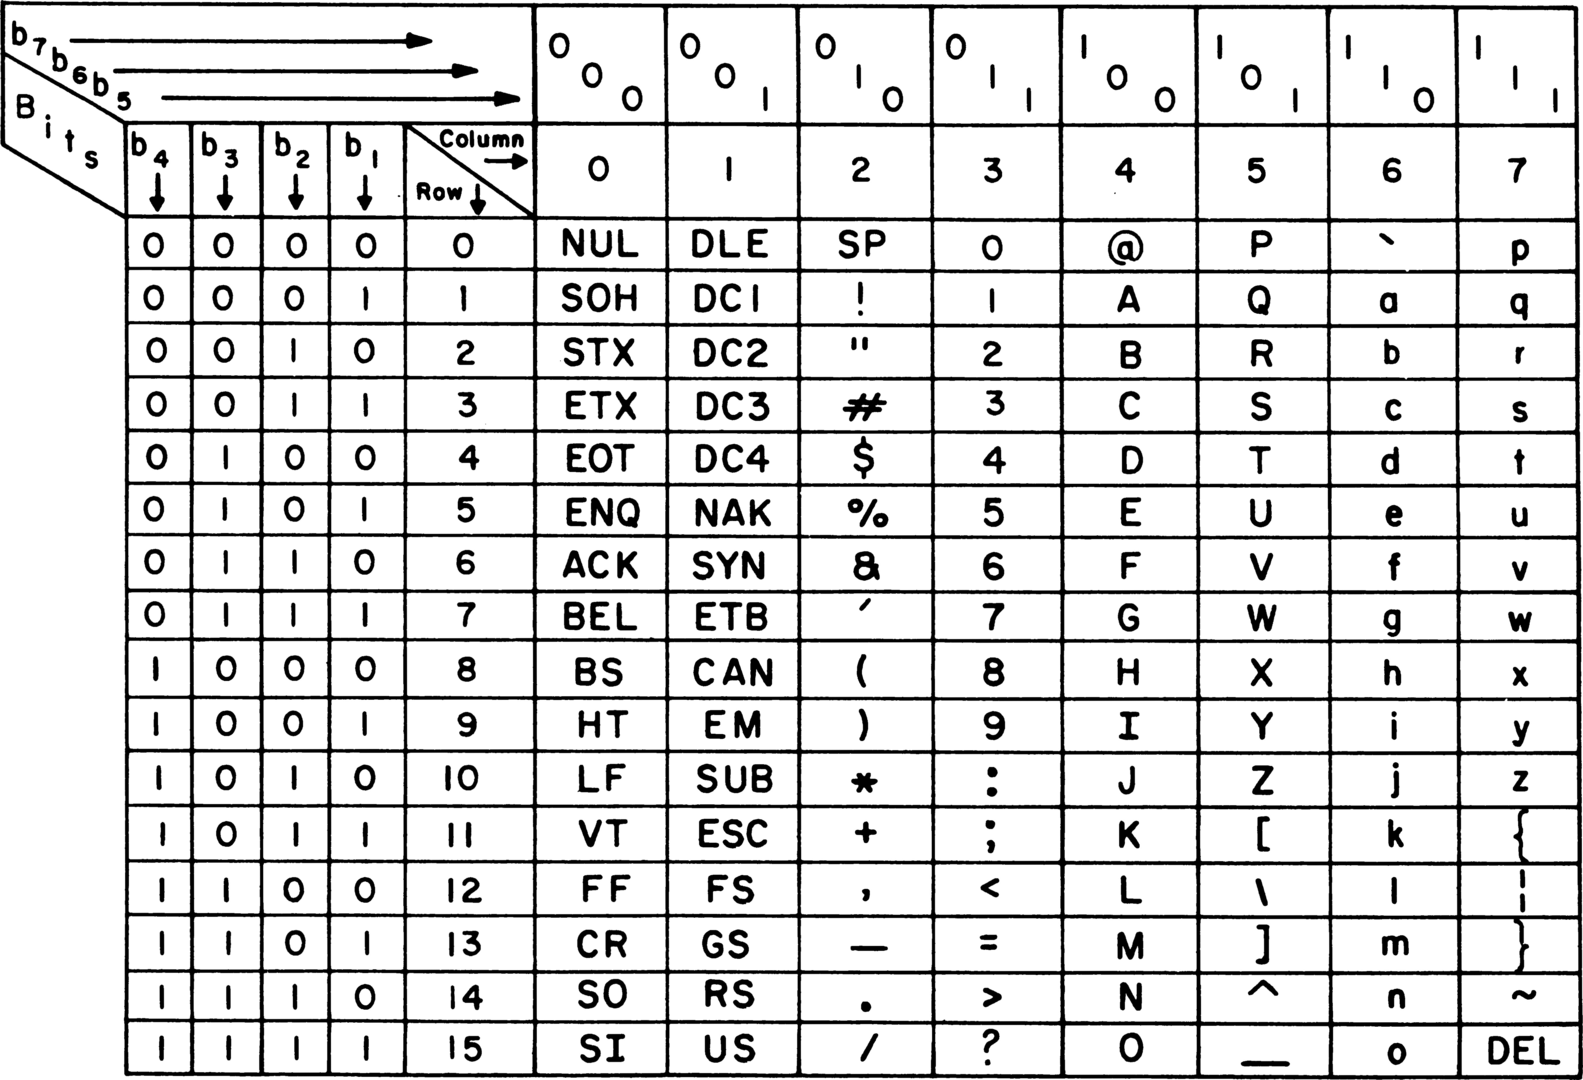
\includegraphics[width=0.75\textwidth]{examples/fig/ASCII.png}
%   \end{center}
%   \begin{flushleft}
%     \vspace{-4mm}
%     \tiny\url{https://de.wikipedia.org/wiki/American\_Standard\_Code\_for\_Information\_Interchange\#/media/Datei:USASCII\_code\_chart.png}
%   \end{flushleft}
% \end{frame}
% \begin{frame}
%   \frametitle{ASCII - Table}
%   This way everything is up to interpretation: 
%   You can read the file as ASCII if there are no special characters in it.:
%   \lstinputlisting[language=python, lastline=5]{examples/ascii.py}
% \end{frame}
% \begin{frame}
%   \frametitle{Using other encodings}
%   With another encoding you can read special characters such as \glq Ö\grq:
%   \lstinputlisting[language=python, firstline=6]{examples/ascii.py}
% \end{frame}
% \section{pickle}
% \begin{frame}
%   \frametitle{pickle}
%   \texttt{\hrefu{https://docs.python.org/3/library/pickle.html}{pickle}} is a module that allows you to store almost any Python object (lists, dictionaries, \dots) in a file.\\
%   \vspace{5mm}
%   \texttt{\hrefu{https://docs.python.org/3/library/pickle.html}{pickle}} is a binary format, so you have to open the file in binary mode (\texttt{wb} or \texttt{rb}).\\
%   \vspace{5mm}
%   Use the \texttt{\hrefu{https://docs.python.org/3/library/pickle.html\#pickle.dump}{dump()}} method to write an object to a file, and the \texttt{\hrefu{https://docs.python.org/3/library/pickle.html\#pickle.load}{load()}} method to read an object from a file.
% \end{frame}
% \begin{frame}
%   \frametitle{pickle -- Example}
%   \lstinputlisting[language=python]{examples/pickle\_example.py}
% \end{frame}
% \section{csv-Import (built-in)}

%%%%%%%%%%%%%%%%%%%%%%%%%%%%%%%%%%%%%%%%%%%%%%%%%%%%%%%%%%%%%%%%%%%%%%%%%%%%

\end{document}
%%%%%%%%%%%%%%%%%%%%%%%%%%%%%%%%%%%%%%%%%%%%%%%%%%%%%%%%%%%%%%%%%%%%%%%%%%%%

%% EOF
